\subsection{Intersegmental Government (IG)}

\subsubsection{Internal structure of consonants}


\paragraph{A (aperture)}
\begin{itemize}
\item nasals \cite[p.~55]{scheer2004}
\item \textquote[{\cite[p.~53]{scheer2004}}]{%
  The prime A co-defines the consonantal identities of the labio-dental and
  the palatoalveolar locus, but is absent from bilabial segments}
\end{itemize}

\paragraph{U}
\textipa{[r,l,n]} \cite[p.~55]{scheer2004}

\paragraph{I}
\textipa{[\c{c}]} (palatalisation of \textipa{[X]})
  \begin{itemize}
  \item genau dann wenn nach Segment mit I
  \item coronale sonoranten \textipa{[n,l,r]} = I-provider
  \end{itemize}
  \cite[p.~56]{scheer2004}

\paragraph{? (occlusion)}

\paragraph{}
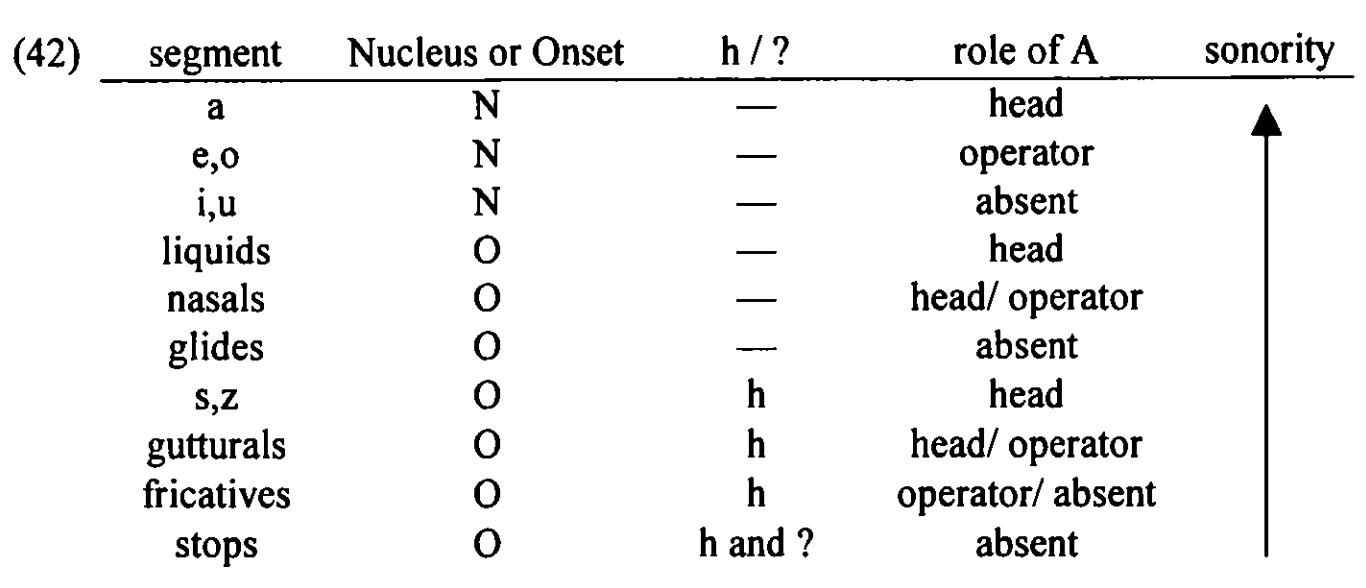
\includegraphics[width=.5\textwidth]{figures/phon-primes-ah-sonority.png}
\cite[p.~52]{scheer2004}

\paragraph{Interaction}
\begin{itemize}
\item \enquote{A and ? hate each other: they cannot compine}\cite[p.~52]{scheer2004}
\end{itemize}